\documentclass[border=12pt]{standalone}
\usepackage{xcolor}
\usepackage{tikz}
\usetikzlibrary{arrows.meta, positioning, calc, fit, backgrounds, decorations.pathreplacing, shapes.geometric}

\definecolor{gold}{HTML}{CFB87C}
\definecolor{dkblue}{HTML}{156082}
\definecolor{ltblue}{HTML}{D0DEE8}
\definecolor{accent2}{HTML}{D9E8F7}
\definecolor{green}{HTML}{196B24}
\definecolor{ltgreen}{HTML}{D4E8D4}
\definecolor{dkgray}{HTML}{333333}
\definecolor{medgray}{HTML}{888888}
\definecolor{ltgray}{HTML}{F2F2F2}
\definecolor{cream}{HTML}{F5F0E6}

\tikzset{
    pbox/.style={
        draw=dkblue, fill=accent2, rounded corners=5pt,
        minimum width=2.8cm, minimum height=1.5cm,
        font=\large\bfseries\color{dkblue}, line width=1.2pt,
        text depth=0pt, align=center,
    },
    outbox/.style={
        draw=green, fill=ltgreen, rounded corners=5pt,
        minimum width=2.8cm, minimum height=1.5cm,
        font=\large\bfseries\color{green}, line width=1.2pt,
        text depth=0pt, align=center,
    },
    arr/.style={
        -{Stealth[length=8pt, width=6pt]}, line width=2pt, gold,
    },
    sweeplabel/.style={
        draw=dkblue!50, fill=dkblue, rounded corners=3pt,
        minimum width=2.0cm, minimum height=0.7cm,
        font=\normalsize\bfseries\color{white}, line width=0pt,
        text depth=0pt, align=center,
    },
    sweepdesc/.style={
        font=\small\color{medgray}, align=center,
    },
    sweeparr/.style={
        -{Stealth[length=5pt]}, dkblue!50, line width=1pt, dashed,
    },
    infobadge/.style={
        draw=medgray!40, fill=ltgray, rounded corners=3pt,
        font=\normalsize\color{dkgray}, line width=0.5pt,
        inner sep=6pt, text depth=0pt, align=center,
    },
}

\begin{document}
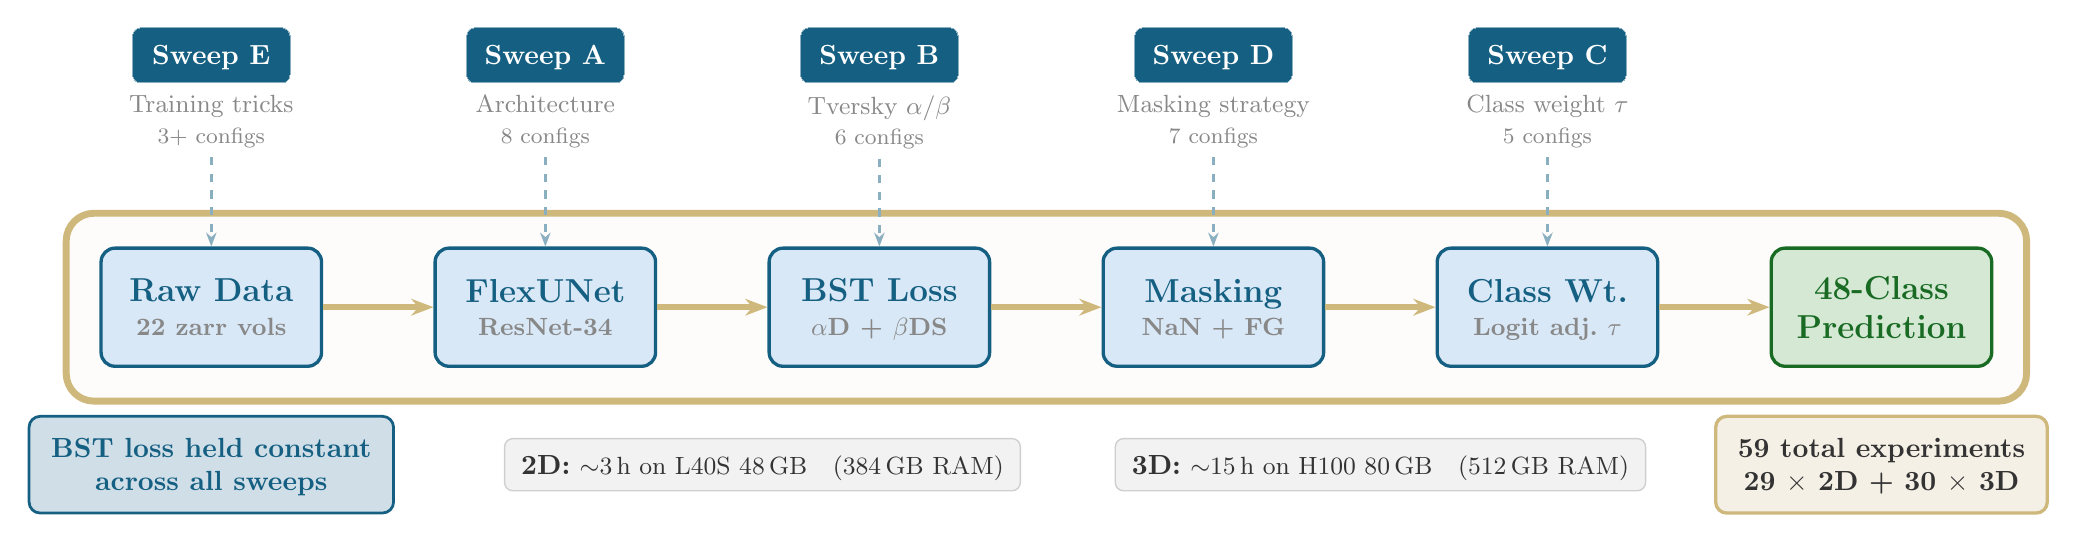
\begin{tikzpicture}[node distance=2.0cm]

% ═══ MAIN PIPELINE ROW (y=0) ═══
\node[pbox] (data) at (0, 0) {Raw Data\\[-2pt]{\small\color{medgray}22 zarr vols}};
\node[pbox, right=1.4cm of data] (model) {FlexUNet\\[-2pt]{\small\color{medgray}ResNet-34}};
\node[pbox, right=1.4cm of model] (loss) {BST Loss\\[-2pt]{\small\color{medgray}$\alpha$D + $\beta$DS}};
\node[pbox, right=1.4cm of loss] (mask) {Masking\\[-2pt]{\small\color{medgray}NaN + FG}};
\node[pbox, right=1.4cm of mask] (weight) {Class Wt.\\[-2pt]{\small\color{medgray}Logit adj.\ $\tau$}};
\node[outbox, right=1.4cm of weight] (out) {48-Class\\Prediction};

% Arrows
\draw[arr] (data) -- (model);
\draw[arr] (model) -- (loss);
\draw[arr] (loss) -- (mask);
\draw[arr] (mask) -- (weight);
\draw[arr] (weight) -- (out);

% Gold highlight border
\begin{pgfonlayer}{background}
\node[draw=gold, line width=2.5pt, rounded corners=10pt, inner sep=12pt,
      fill=gold!4,
      fit=(data)(model)(loss)(mask)(weight)(out)] {};
\end{pgfonlayer}

% ═══ SWEEP LABELS (above, pointing down) ═══
\node[sweeplabel] (sA) at ([yshift=3.2cm]model) {Sweep A};
\node[sweepdesc, below=1pt of sA] (sAd) {Architecture\\{\footnotesize 8 configs}};

\node[sweeplabel] (sB) at ([yshift=3.2cm]loss) {Sweep B};
\node[sweepdesc, below=1pt of sB] (sBd) {Tversky $\alpha/\beta$\\{\footnotesize 6 configs}};

\node[sweeplabel] (sC) at ([yshift=3.2cm]weight) {Sweep C};
\node[sweepdesc, below=1pt of sC] (sCd) {Class weight $\tau$\\{\footnotesize 5 configs}};

\node[sweeplabel] (sD) at ([yshift=3.2cm]mask) {Sweep D};
\node[sweepdesc, below=1pt of sD] (sDd) {Masking strategy\\{\footnotesize 7 configs}};

% Sweep E goes to model (training tricks)
\node[sweeplabel] (sE) at ([yshift=3.2cm]data) {Sweep E};
\node[sweepdesc, below=1pt of sE] (sEd) {Training tricks\\{\footnotesize 3+ configs}};

% Dashed arrows from sweep labels to pipeline boxes
\draw[sweeparr] (sAd.south) -- (model.north);
\draw[sweeparr] (sBd.south) -- (loss.north);
\draw[sweeparr] (sCd.south) -- (weight.north);
\draw[sweeparr] (sDd.south) -- (mask.north);
\draw[sweeparr] (sEd.south) -- (data.north);

% ═══ COMPUTE BADGES (below pipeline) ═══
% Position all four badges as: BST | 2D | 3D | 59 experiments
\node[draw=dkblue, fill=ltblue, rounded corners=4pt, line width=1pt,
      font=\normalsize\bfseries\color{dkblue}, inner sep=8pt,
      text depth=0pt, align=center]
    (bst_badge) at ([yshift=-2.0cm]data)
    {BST loss held constant\\across all sweeps};

\node[infobadge]
    (badge_2d) at ([yshift=-2.0cm]$(model)!0.65!(loss)$)
    {\textbf{2D:} \raisebox{0pt}{\small$\sim$3\,h on L40S 48\,GB\quad (384\,GB RAM)}};

\node[infobadge]
    (badge_3d) at ([yshift=-2.0cm]$(mask)!0.5!(weight)$)
    {\textbf{3D:} \raisebox{0pt}{\small$\sim$15\,h on H100 80\,GB\quad (512\,GB RAM)}};

% 59 experiments badge
\node[draw=gold, fill=cream, rounded corners=4pt, line width=1.2pt,
      font=\normalsize\bfseries\color{dkgray}, inner sep=8pt,
      text depth=0pt, align=center]
    at ([yshift=-2.0cm]out)
    {59 total experiments\\29 $\times$ 2D + 30 $\times$ 3D};

\end{tikzpicture}
\end{document}
